% !TeX spellcheck = en_US

% Kompatibilität zu Libs
% DBs zu hohe Latenz
% Der Plan = GIS Layer
\chapter{Software Design}
\label{sec:software_design}
This chapter discusses the current state and possible solutions for working with GIS inside the LIFE simulation system.



\section{Current state}
Currently the GIS support inside MARS is partial, some components of the environment are capable of handling GIS, while others are not supporting it yet.


\subsection{WebUI}
The WebUI supports GIS for importing and managing this kind of data. It's successor the teaching UI currently does not support GIS. Due to the micro-service structure of the back-end services it is possible for the front-ends to coexist until the feature has been implemented.

\subsection{Back-end Services}
The back-end services fully support GIS. The file service accepts the uploaded files and hands control over to the GIS Data Service (GDS). 

\subsubsection{GIS Data Service}
The GDS is capable of handling the most common GIS types, these are GeoTIFF, GeoJSON and Esri ASCII Grid for raster and Shapefile for vector files. The files may be provided compressed inside a .zip file or as plain files.\\
During the import the GDS determines the type of data automatically by checking the file extension. Once detected, the file is validated and the spatial reference is determined. In case of a valid geo-referenced input, the file is imported into the GeoServer for persistence.


\subsubsection{GeoServer} \label{sec:GS}
The GeoServer is an open source software that is tailored to store, manage and share GIS. It offers a web GUI as well as a REST API for interaction. The API is structured in a way that it implements common Open Geospatial Consortium (OGC) standards for retrieving data.\\
The Web Feature Service (WFS) allows to retrieve features of vector data, Web Coverage Service (WCS) enables downloading raster data and the Web Map Service (WMS) can generate a tile map for viewing GIS on a map.\\
The GeoServer is build for working with few files and a small number of users. The MARS use-case requires to read thousands to millions of single values in parallel in a short amount of time. The GeoServer does not satisfy this demands. The retrieval of single values is not supported, since the general use-case is to work with complete files and the performance for retrieving data is very poor which will require a better solution.\\
figure \ref{img:gs-read-performance} emphasizes this. It shows GeoServer response time for different storage solutions. All values exceed one second which is not expectable for the amount of requests needed for this work. \cite{Pandey2016} argues that disk-based systems are generally not fast enough for real-time analysis.

\begin{figure}[H]
	\centering
	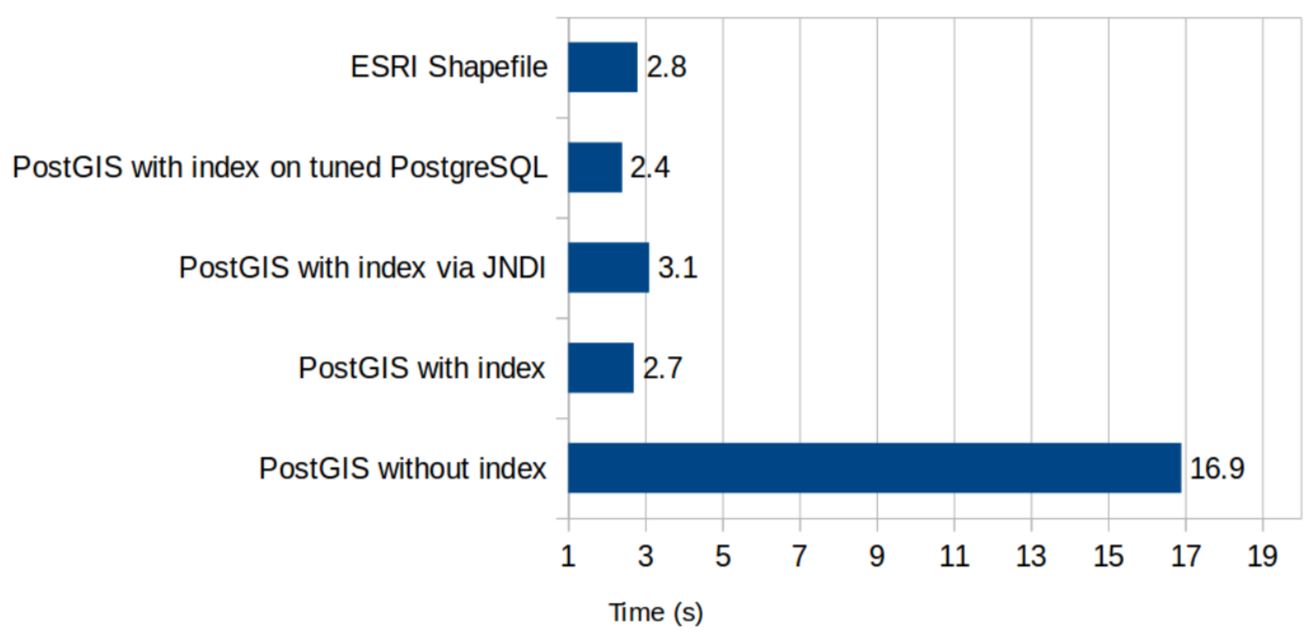
\includegraphics[width=0.8\columnwidth]{res/gs-read-performance}\\
	\caption[]{GeoServer average time of response by \cite{ruuvzivcka2016comparing}}
	\label{img:gs-read-performance}
\end{figure}

\subsection{LIFE -- GIS Layer}
The GIS Layer inside MARS LIFE reads the data provided by the GDS and uses it inside the simulation. Since the migration from C\# to .NET Core inside LIFE the GIS layer is not compatible anymore.\\
The current models therefore do not leverage GIS for their input. Data is being transfered into other formats to work around these shortcomings. Vector data is mainly represented as comma separated values (.csv) files and raster data are represented in custom formats.


\section{Solutions}
As mentioned in section \ref{sec:GS} reading data from the GeoServer during the simulation is not feasible inside a high performance environment. Figure \ref{img:spatial-queries} shows that local GIS libraries tend to drastically outperform database solutions. For this reason local libraries were also considered during the evaluation.\\
Hadoop-GIS with MapReduce as suggested by \cite{Wang2011} offers very good scalability but does not support the hight IO and low latency focused use-case of the MARS system.  GeoMesa and Vector Cluster as suggested by \cite{Toups2016} was not taken into closer consideration, since PostGIS offered a better performance. Vertica and DBMS-X as proposed by \cite{Pavlo2009} were ruled out du to lack of promising performance. \\
Table \ref{fig:feature_comparison} shows an overview of the technologies which have been considered to be beneficial. The main criteria for choosing these libraries and databases were geospatial capabilities, compatibility to .NET Core and performance.

\begin{figure}[H]
	\centering
	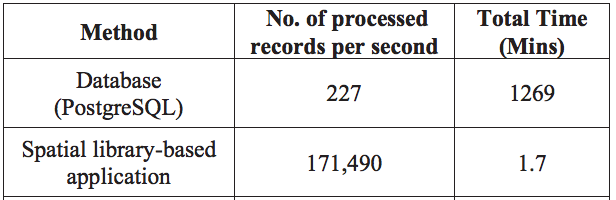
\includegraphics[width=0.6\columnwidth]{res/spatial-queries}\\
	\caption[]{Processing time on spatial queries by \cite{Witayangkurn2012}}
	\label{img:spatial-queries}
\end{figure}

\begin{table}[H]
	\caption{GIS solutions feature comparison}
	\label{fig:feature_comparison}
	\begin{tabular}{|l|l|l|l|}
	\hline \textbf{Name}	& \textbf{Raster support} & \textbf{Vector support} & \textbf{Type}\\
	\hline GeoServer & Yes & Yes & Self-hosted product\\
	\hline PostGIS	& Yes* & Yes & PostgreSQL DB + GIS ext.\\
	\hline MongoDB	& No & Yes & DB with spatial capabilities\\
	\hline Dotspatial & Yes & Yes & C\# library\\
	\hline NetTopologySuite	& No & Yes & C\# library\\
	\hline AsciiGridParser & Yes & No & Own .NET Core Component\\
	\hline
	\end{tabular}
	\caption*{ \raggedright * Large file failed.}
\end{table}

All mentioned technologies were performance tested with the same input files. A small, medium and a large size vector and raster file. The sizes were 10 KB, 6.5 MB and 105 MB. Each test performs 1,000 parallel reads and the result is the average of three separate tests. 
The results are listed in figure \ref{fig:vector_performace} for vector and \ref{fig:raster_performace} for raster inputs.

\begin{figure}[H]
	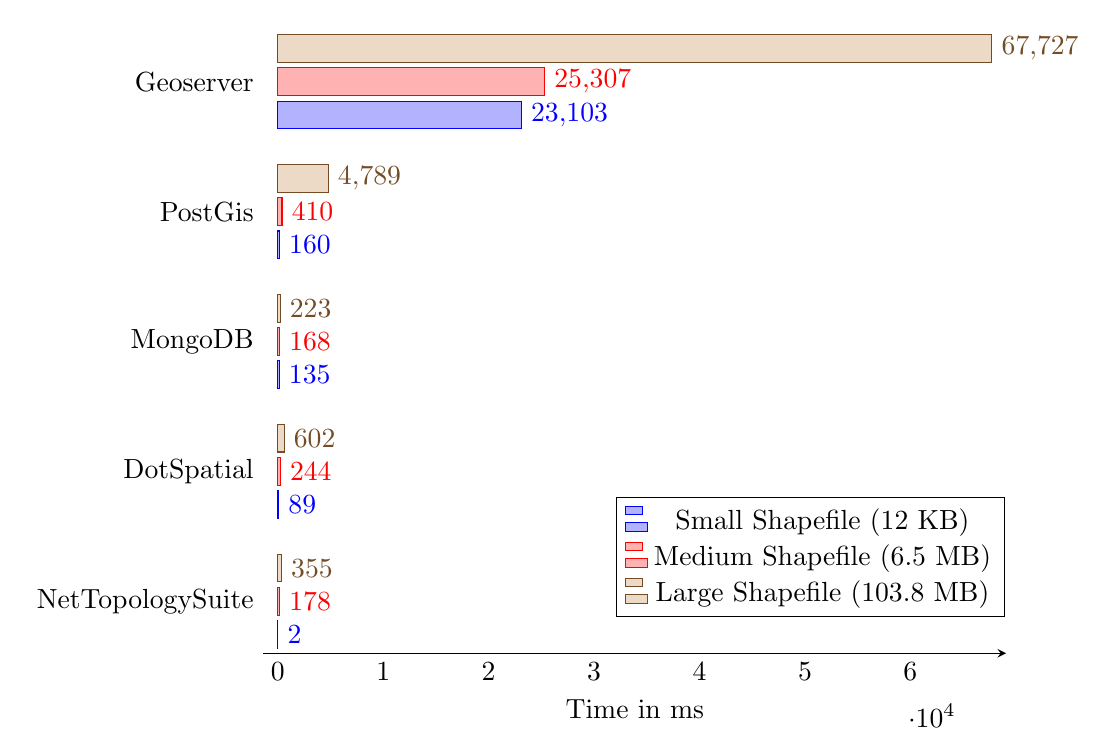
\begin{tikzpicture}
	\begin{axis}[
	xbar,
	y axis line style = { opacity = 0 },
	axis x line       = bottom,
	tickwidth         = 0pt,
	%	enlarge y limits  = 0.02,
	enlarge x limits  = 0.02,
	symbolic y coords = {NetTopologySuite, DotSpatial, MongoDB, PostGis, Geoserver},
	nodes near coords,
	height=9.5cm,
	legend style={at={(0.737,0.25)},anchor=north},
	xlabel={Time in ms},
	]
	% Small Shapefile
	\addplot coordinates {
		(23103,Geoserver)
		(160,PostGis)
		(135,MongoDB)
		(89,DotSpatial)
		(2,NetTopologySuite)
	};
	% Mid Shapefile
	\addplot coordinates {
		(25307,Geoserver)
		(410,PostGis)
		(168,MongoDB)
		(244,DotSpatial)
		(178,NetTopologySuite)
	};
	% Large Shapefile
	\addplot coordinates {
		(67727,Geoserver)
		(4789,PostGis)
		(223,MongoDB)
		(602,DotSpatial)
		(355,NetTopologySuite)
	};
	\legend{Small Shapefile (12 KB),Medium Shapefile (6.5 MB),Large Shapefile (103.8 MB)}
	\end{axis}
	\end{tikzpicture}
	\caption{Vector performance for 1k reads}
	\label{fig:vector_performace}
\end{figure}


\begin{figure}[H]
	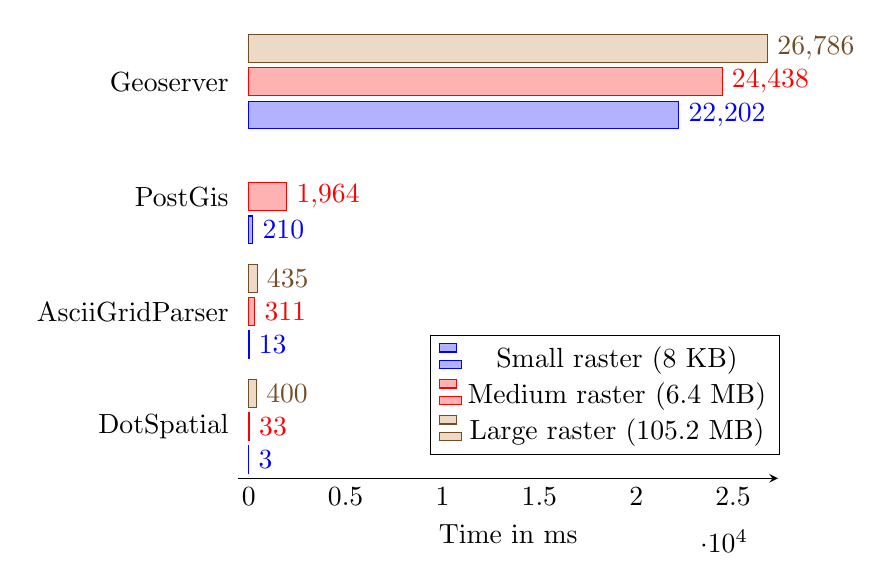
\begin{tikzpicture}
	\begin{axis}[
	xbar,
	y axis line style = { opacity = 0 },
	axis x line       = bottom,
	tickwidth         = 0pt,
	enlarge y limits  = 0.15,
	enlarge x limits  = 0.02,
	symbolic y coords = {DotSpatial, AsciiGridParser, PostGis, Geoserver},
	nodes near coords,
	legend style={at={(0.68,0.32)},anchor=north},
	xlabel={Time in ms},
	]
	% Small Rasterfile
	\addplot coordinates {
		(22202,Geoserver)
		(210,PostGis)
		(13,AsciiGridParser)
		(3,DotSpatial)
	};
	% Mid Rasterfile
	\addplot coordinates {
		(24438,Geoserver)
		(1964,PostGis)
		(311,AsciiGridParser)
		(33,DotSpatial)
	};
	% Large Rasterfile
	\addplot coordinates {
		(26786,Geoserver)
		(nan,PostGis) % 342197
		(435,AsciiGridParser)
		(400,DotSpatial)
	};
	\legend{Small raster (8 KB),Medium raster (6.4 MB),Large raster (105.2 MB)}
	\end{axis}
	\end{tikzpicture}
	\caption{Raster performance for 1k reads}
	\label{fig:raster_performace}
\end{figure}


\subsection{PostGIS}
PostGIS is a PostgreSQL database with GIS extensions. It supports storing vector data as well as raster data.\\
The performance is way better than the of the GeoServer, however PostGIS did not handle the large file very well. The reading of the large vector file took over 10 times longer than the smaller file, which is surprising since the data is broken into tables. A larger table should not effect the response time by that extend.\\
The big raster file was even worse. The test crashed with an OutOfMemory exception on a machine with 16 GB of RAM. Limiting the parallelism of threads to 7 worked, but the results of around ~340,000 ms (5 min. 40 sec.) were not acceptable.


\subsection{MongoDB}
MongoDB offeres good overall performance for vector data. The file size does not effect the overall performance by a large extend. For the medium and large file it was even faster than NetTopologySuite (NTS). Raster GIS is not supported.\\
Figure \ref{img:mongo-vs-postgres} shows the performance of MongoDB compared to PostgreSQL for vector GIS.

\begin{figure}[H]
	\centering
	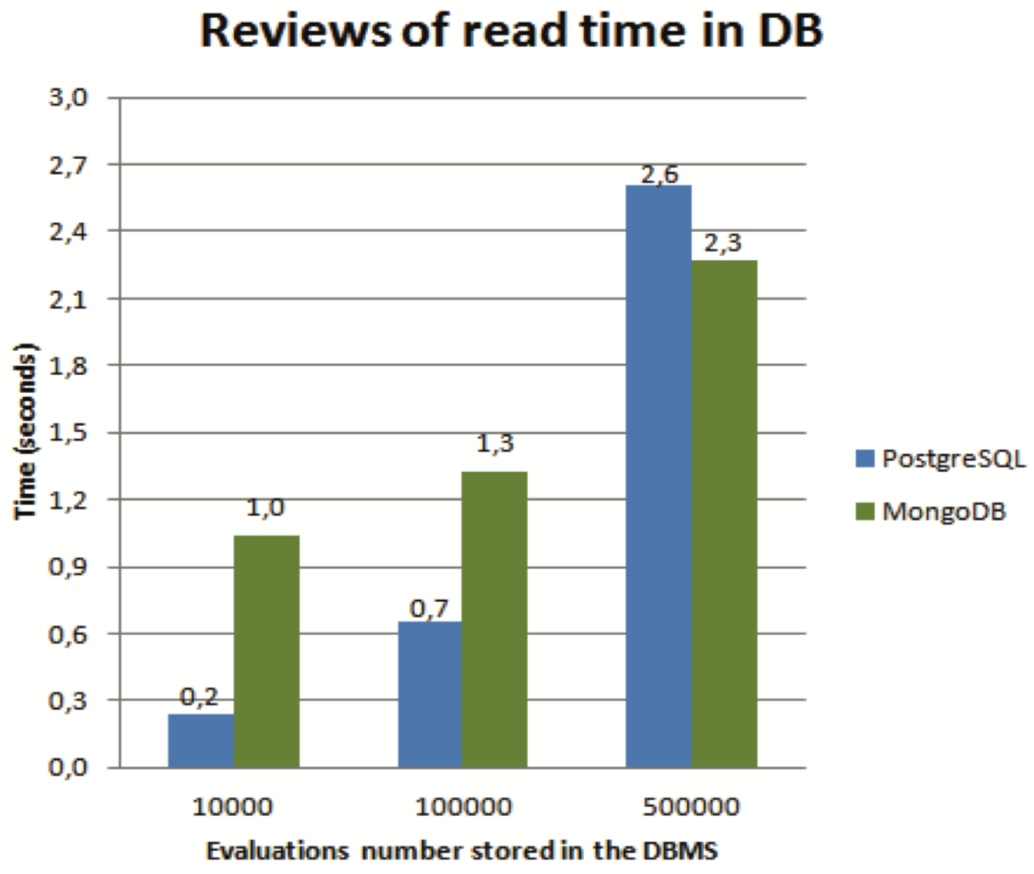
\includegraphics[width=0.6\columnwidth]{res/mongo-vs-postgres}\\
	\caption[]{Comparison of the times of the read of the evaluation data in the Database PostgreSQL and MongoDB by \cite{Maia2016}}
	\label{img:mongo-vs-postgres}
\end{figure}

\subsection{DotSpatial}
DotSpatial offers average vector read performance. MongoDB and NTS perform slightly better. Since both these technologies are not available for raster GIS, DotSpatial performs best in that field.\\
As of August 25th 2017 the library has not been ported to .NET Core. This is why a .NET Core compatible Esri AsciiGridParser was created.\\


\subsection{NetTopologySuite}
NTS has the best vector read performance. It is not available for raster GIS. As of August 2017 NTS is available for .NET Core. The implementation of the Shapefile compatibility is currently missing, but expected to return soon.\\


\subsection{AsciiGridParser}
Since DotSpatial is not ported to .NET Core yet, there is no acceptable solution for reading raster GIS during the simulation. This is, why the author of this work created a parser for Esri's ASCII grid format.\\
ASCII grid is a text-based, geo-referenced raster format that other raster formats like GeoTIFF can be converted into. Due to the text-based nature of the format the read performance is not as good as the DotSpatial reader. It is however within the same range and offers very good performance until DotSpatial gets migrated.



\section{Results}
The performance measurement for the local libraries (NTS, DotSpatial and the AsciiGridParser) are different to the database solutions. These libraries open the file into RAM and read from it. The opening takes majority of the time, while reads from RAM is much faster. Since the file can be loaded once and read from during the simulation, the time increase for additional reads is very low, making these solution preferable at scale.\\
The additional performance tests in \ref{fig:vector_performace_best} and \ref{fig:raster_performace_best} with 10k reads verify this. The read times for local libraries is increased by a few milliseconds, while MongoDB and PostGis take almost 10 times as much time. With agent counts in the millions, the described effect becomes even more extreme, in favor of NTS, DotSpatial and the AsciiGridParser.

\begin{figure}[H]
	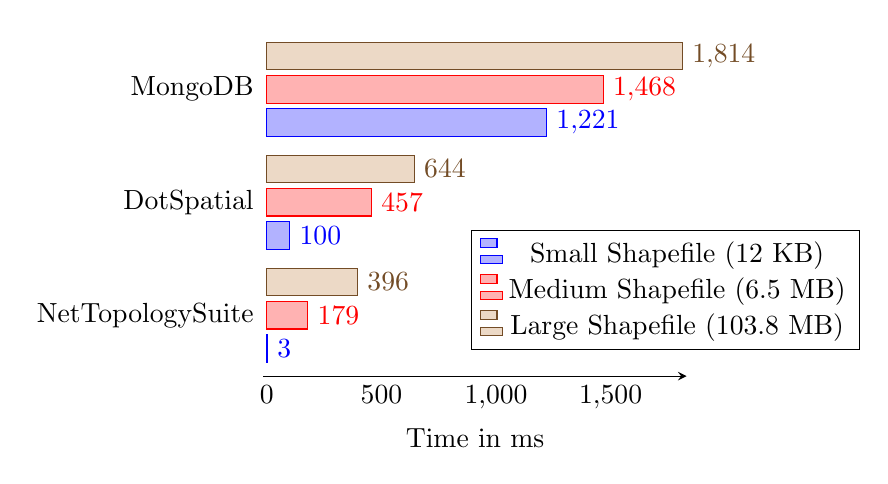
\begin{tikzpicture}
	\begin{axis}[
	xbar,
	y axis line style = { opacity = 0 },
	axis x line       = bottom,
	tickwidth         = 0pt,
	enlarge y limits  = 0.27,
	enlarge x limits  = 0.01,
	symbolic y coords = {NetTopologySuite, DotSpatial, MongoDB},
	ytick=data,
	nodes near coords,
	height=6cm,
	legend style={at={(0.95,0.42)},anchor=north},
	xlabel={Time in ms},
	]
	% Small Shapefile
	\addplot coordinates {
		(1221,MongoDB)
		(100,DotSpatial)
		(3,NetTopologySuite)
	};
	% Mid Shapefile
	\addplot coordinates {
		(1468,MongoDB)
		(457,DotSpatial)
		(179,NetTopologySuite)
	};
	% Large Shapefile
	\addplot coordinates {
		(1814,MongoDB)
		(644,DotSpatial)
		(396,NetTopologySuite)
	};
	\legend{Small Shapefile (12 KB),Medium Shapefile (6.5 MB),Large Shapefile (103.8 MB)}
	\end{axis}
	\end{tikzpicture}
	\caption{Vector performance for 10k reads}
	\label{fig:vector_performace_best}
\end{figure}

\begin{figure}[H]
	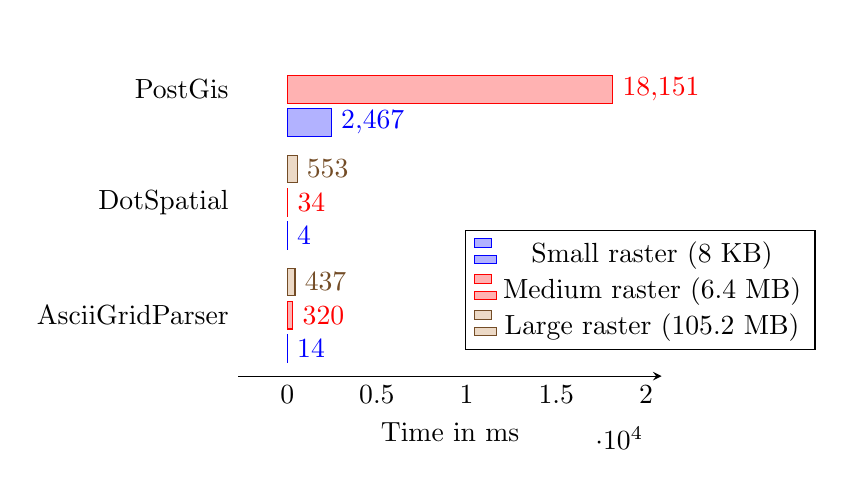
\begin{tikzpicture}
	\begin{axis}[
	xbar,
	y axis line style = { opacity = 0 },
	axis x line       = bottom,
	tickwidth         = 0pt,
	enlarge y limits  = 0.27,
	enlarge x limits  = 0.15,
	symbolic y coords = {AsciiGridParser, DotSpatial, PostGis},
	ytick=data,
	nodes near coords,
	height=6cm,
	legend style={at={(0.95,0.42)},anchor=north},
	xlabel={Time in ms},
	]
	% Small Raster
	\addplot coordinates {
		(2467,PostGis)
		(4,DotSpatial)
		(14,AsciiGridParser)
	};
	% Mid Raster
	\addplot coordinates {
		(18151,PostGis)
		(34,DotSpatial)
		(320,AsciiGridParser)
	};
	% Large Raster
	\addplot coordinates {
		(nan,PostGis)
		(553,DotSpatial)
		(437,AsciiGridParser)
	};
	\legend{Small raster (8 KB),Medium raster (6.4 MB),Large raster (105.2 MB)}
	\end{axis}
	\end{tikzpicture}
	\caption{Raster performance for 10k reads}
	\label{fig:raster_performace_best}
\end{figure}
